\section{Content Addressable Parallel Processor}
The circuitry of a CAPP can be broken down into 3 main parts. The tags, the cells and the search registers. 
The search registers are the least complex circuits in a CAPP. They consist of 2 different registers, the comparand and the mask. 
The comparand is the word to search for, and the mask contains locations of bits in the word to ignore during the search.
The design for these are given in figure \ref{search_circuit}.

\begin{figure}
  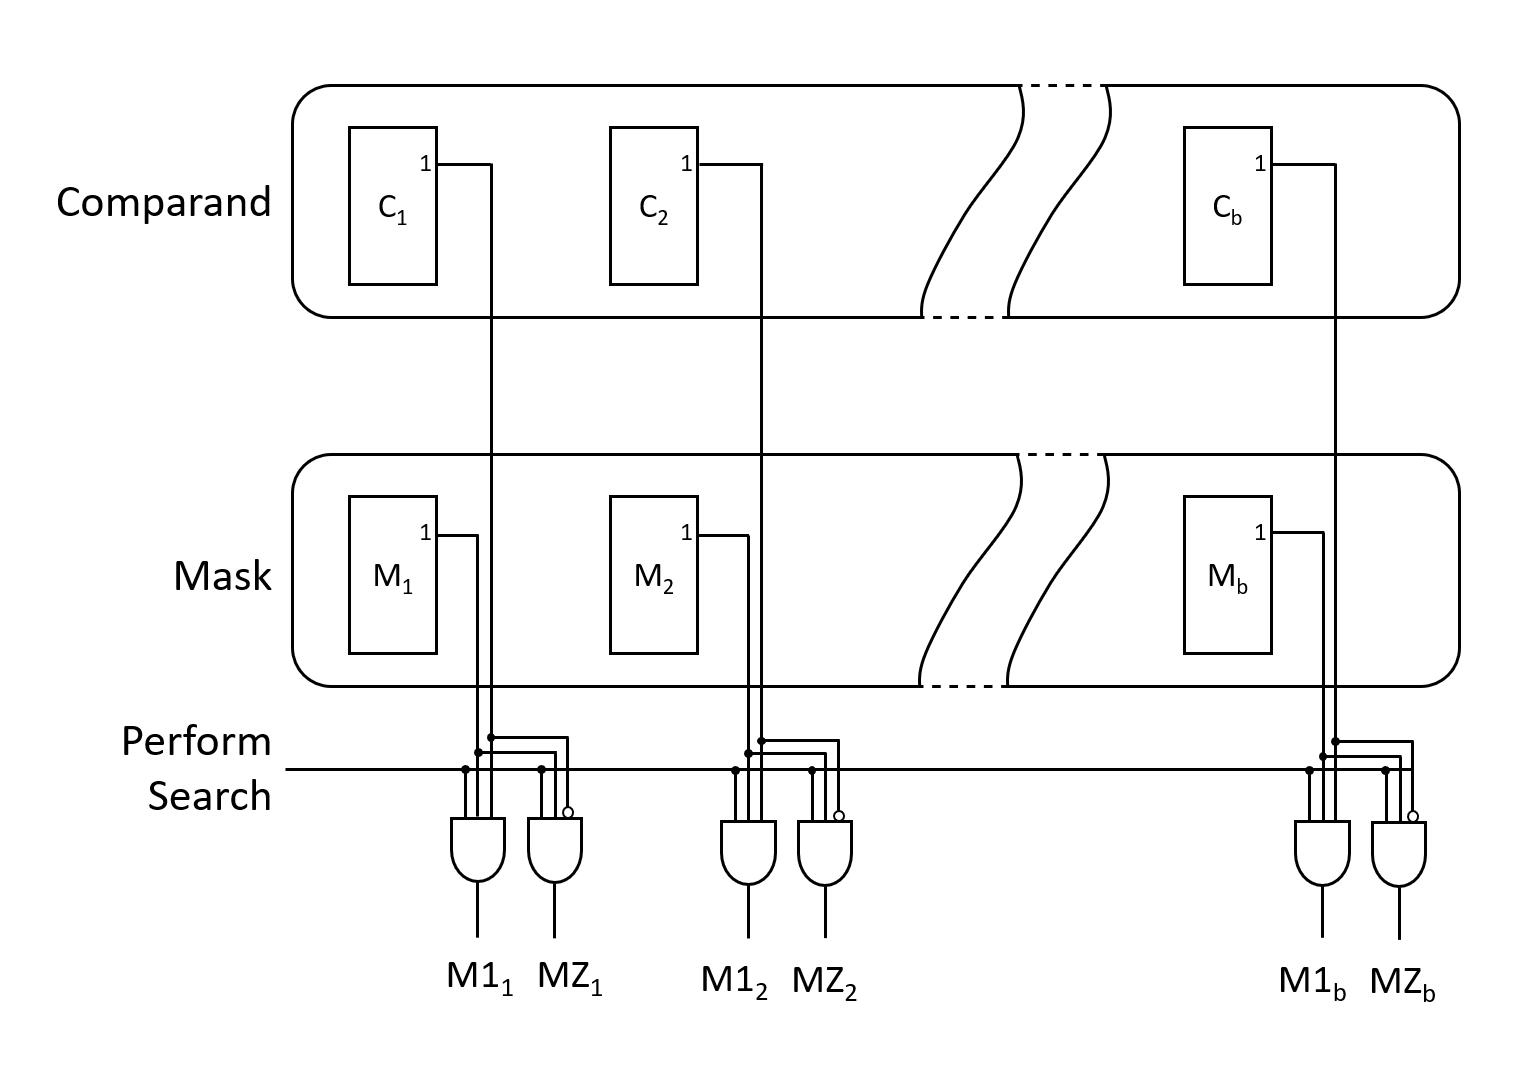
\includegraphics[height=5cm]{FPGA-CAPP research paper/images/search_registers.png}
  \caption{Design of the CAPP search registers}
  \label{search_circuit}
\end{figure}

The second most complex circuitry is found in the tags. Tags are bits for all cells, if the bit of a cell is high after a search, it means that the word in that cell was found in the search. In other words, after a search, the cells with high tag bits are the ones that were found. As all the tag bits of a CAPP have to change in constant time (i.e. in parallel), match lines from the search registers go through each cell to create mismatch lines which turn irrelevant tags off whenever the search signal is set. The circuitry also includes logic for manually setting all bits high and selecting the first tag bit that is on. The design for these are given in Figure \ref{tag_registers}.

\begin{figure}
  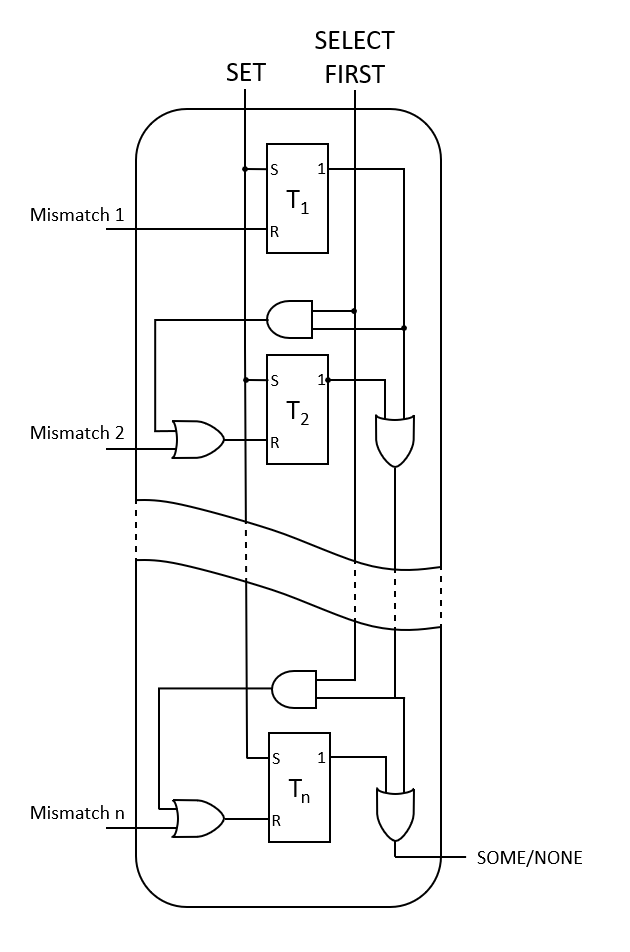
\includegraphics[height=14cm]{FPGA-CAPP research paper/images/tag_registers.png}
  \caption{Design of the CAPP tag registers}
  \label{tag_registers}
\end{figure}

Arguably the most complex circuitry is found in the memory cells themselves, as it encapsulates the main logic for writing, reading and searching. 
Each bit of each cell is surrounded by 2 write lines, 2 search lines and 1 read line. The nth bits of all cells share these lines.
The value of each bit in each cell is changed to 0 or 1 depending on which write line is set high. Conversely, depending on the 2 search lines and the bit value, a mismatch line that is connected to the tag bit of the cell is set high or low  \ref{mismatch_lines}. This allows the CAPP to search or write in parallel. The output of all the read lines is the bitwise OR of all cells that have their tag bits on as shown in Figure \ref{read_lines}. 

\begin{figure}
  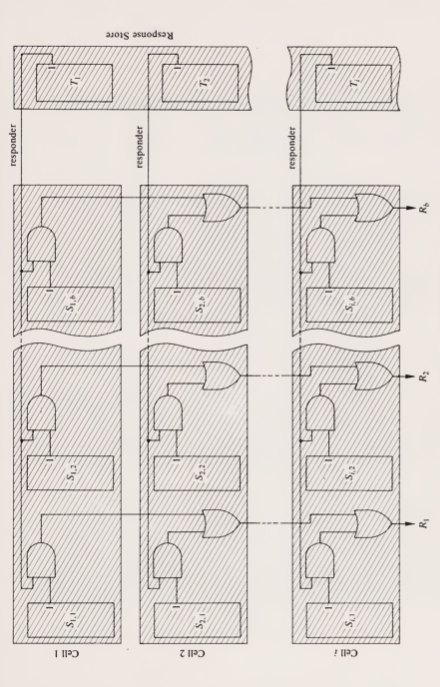
\includegraphics[height=13cm]{FPGA-CAPP research paper/images/read_lines.png}
  \caption{Design of the CAPP tag registers}
  \label{read_lines}
\end{figure}

\begin{figure}
  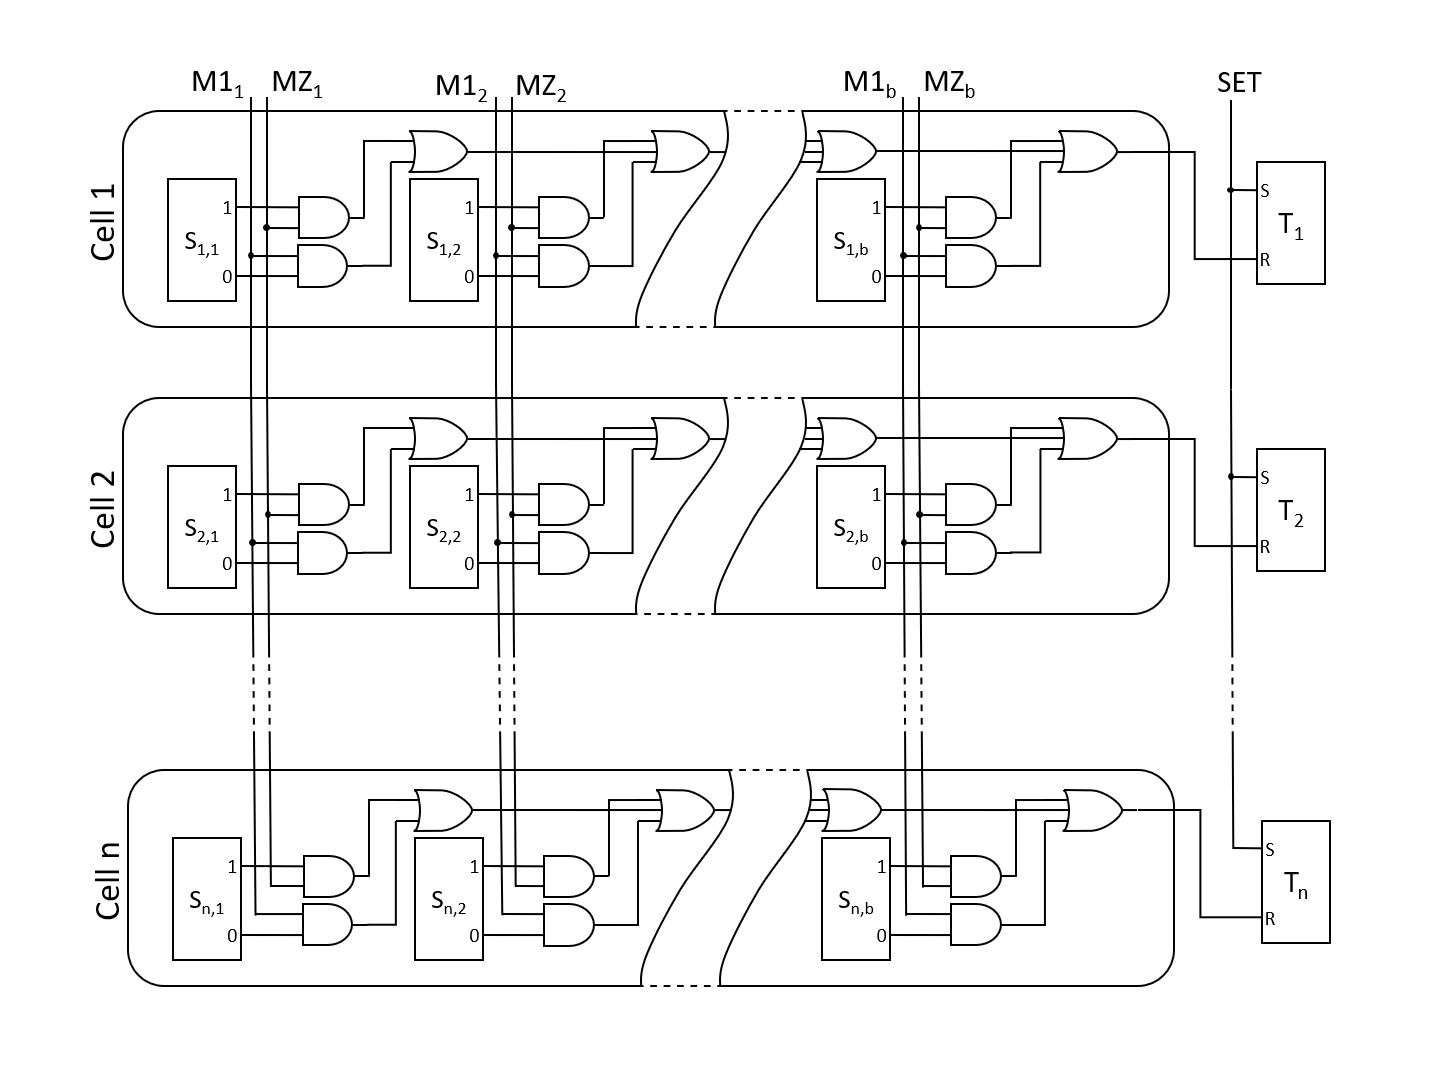
\includegraphics[height=12cm]{FPGA-CAPP research paper/images/mismatch_lines.png}
  \caption{Design of the CAPP tag registers}
  \label{mismatch_lines}
\end{figure}

Clearly, the aforementioned design constitutes a direct translation to Verilog of the introductory CAPP described in Caxton Foster's seminal book on the topic of CAPPs \cite{capp}.
We then used nextpnr for the placing and routing of our Verilog design. The choice of nextpnr was due to its ability to take into timing constraints which were important for the correct implementation of the Serial UART module which needed to function reliably despite being connect to a CAPP module which requires potentially more than one clock cycle to execute a request communicated from the host computer. The resulting layout was synthesized and tested on the TinyFPGA-BX using a Python-based driver to communicate with the resulting USB-CAPP device.
The Finite State Machine at the core of the communication protocol between the host computer and the CAPP is described in the next section.